 \section{Introduction}


\begin{figure}[t]
\centering
% \vskip -0.15in
\centering
{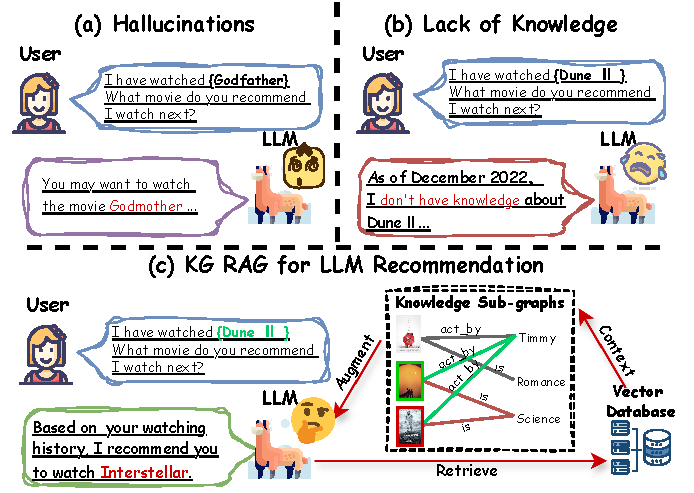
\includegraphics[width=0.98\linewidth]{figures/illustration1.pdf}}
% \vskip -0.1in
% 
\caption{
Illustration of the issues of hallucinations and lack of domain-specific knowledge in LLM-based recommender systems and how they can be addressed by knowledge graph retrieval-augmented generation (KG RAG). } 
\label{fig:illustration}
\vskip -0.2in
\end{figure}
 
Recommender systems, as techniques designed to assist people in making decisions in their daily lives, are increasingly gaining impact in various fields~\citep{kenthapadi2017personalized,he2020lightgcn,fan2019graph}, such as online shopping, job matching, and social media.
Recently, Large Language Models (LLMs) have achieved significant breakthroughs, which further drive developments in various domains~\citep{fan2024graph,zhao2024recommender,wu2023next}. Especially with the success of LLMs, recommender systems have seen rapid growth~\citep{geng2022recommendation,bao2023tallrec,qu2024tokenrec}. By training on a wide range of data, LLMs (e.g., GPT-4~\citep{achiam2023gpt} and LLaMA~\citep{touvron2023llama}) are able to acquire extensive knowledge and demonstrate exceptional language understanding capability.
This capability enables LLM-based recommender systems to capture user preferences through a nuanced understanding of relevant attributes (e.g., user profiles, item descriptions, historical interactions) for more accurate recommendations. 
As a result, LLM-based recommender systems have emerged as a new paradigm in recommendation technology~\citep{zhao2024recommender}.




However, despite their powerful language understanding and generalization capability, LLM-based recommender systems face significant challenges, including hallucinations and lack of up-to-date and domain-specific knowledge~\citep{luo2023reasoning}. 
Specifically, one key issue is that LLM-based recommender systems may generate recommendations that are entirely fictional due to the inherent limitations of LLMs.
For example, an LLM-based recommender system may recommend \textit{"Godmother"}, a non-existent film, to the user who has watched \textit{"The Godfather"}, as illustrated in Figure~\ref{fig:illustration} (a). 
Additionally, LLMs usually lack up-to-date knowledge, which can prevent them from recommending the latest films or products in a timely manner. 
As illustrated in Figure~\ref{fig:illustration} (b), the LLM-based recommender system is unable to recommend the latest films due to the training data only containing up to December 2022. 
Furthermore, LLMs often lack domain-specific knowledge, as recommendation-oriented corpora are very limited during the training phase of LLMs~\citep{geng2022recommendation}. 
Consequently, LLMs may struggle to meet the nuanced needs of recommendation tasks. 
To alleviate these issues, one potential solution is to frequently fine-tune the LLMs with up-to-date and domain-specific knowledge. However, the massive parameters of LLMs make this process computationally expensive and time-consuming, which severely hinders the practical application in the real world.







More recently, Retrieval-Augmented Generation (\textbf{RAG}) leveraging external databases to provide specific knowledge shows promise to solve these problems~\citep{fan2024survey,gao2023retrieval}.
By incorporating an external knowledge base, RAG can retrieve relevant and up-to-date information to complement the LLM's inherent knowledge, thereby mitigating the issues of hallucinations and knowledge gaps~\citep{khandelwal2019generalization,min2020ambigqa,li2024empowering}. This makes RAG a promising technique for enabling LLMs to provide effective recommendations without the need for costly fine-tuning~\citep{ram2023context}.

Despite this potential, vanilla RAG methods that rely on documents and paragraphs often introduce unnecessary noise and even harmful disturbance, which can negatively impact the accuracy and reliability of recommendations~\citep{he2024g}. 
In addition, the structural relationships between entities are overlooked in typical RAG, resulting in the sub-optimal reasoning capability of LLM-based recommender systems~\citep{luo2023reasoning}.
To address the limitations, a prospective solution is to incorporate structured knowledge such as \emph{items' knowledge graph (KG)} to help improve recommendation performance. 
Specifically, KGs offer structured, factual, and editable representations of knowledge, which can provide a faithful knowledge source for recommendations.
As shown in Figure~\ref{fig:illustration} (c), retrieving structured knowledge from the KG can significantly enhance the recommendation capabilities of LLM-based recommender systems.

However, it is challenging to effectively retrieve KGs to enhance the recommendation capabilities of LLMs.
First, KGs store rich factual knowledge in a structured format.
Simply retrieving the triplets or first-order neighbors of an entity (i.e., item) with semantic information neglects the importance of these higher-order neighborhood effects among entities/items, resulting in sub-optimal recommendation performance.
Second, indiscriminate retrieving for each item, regardless of whether the retrieval is necessary or the content is relevant, can degrade the performance of the recommendation while severely reducing the model's efficiency~\citep{asai2023self,labruna2024retrieve}.
Furthermore, structured data in KGs is typically encoded for LLM in the form of serialized text~\citep{wu2023retrieve,sun2023think}, which is insufficient for fully exploiting the structural information inherent in the data~\citep{perozzi2024let,fatemi2023talk}.
Therefore, it is crucial to explore more effective and expressive ways of representing structured data, allowing LLMs to effectively leverage the structure information of retrieved knowledge sub-graphs for recommendations. 


To address the aforementioned challenges, in this paper, we propose a knowledge retrieval-augmented recommendation framework, namely \textbf{K-RagRec}, to provide up-to-date and reliable knowledge by retrieving relevant knowledge from item's KGs for recommendation generation in the era of LLMs. 
Specifically, our proposed framework first performs knowledge sub-graph indexing on the items' KG at a coarse and fine granularity to construct the knowledge vector database. 
Next, a popularity selective retrieval policy is designed to determine which items should be retrieved, followed by the retrieval of specific sub-graphs from the knowledge vector database. 
To refine the quality of retrieval and ensure the most relevant results are prioritized at the top of the input, we subsequently re-rank the retrieved knowledge sub-graphs. 
Finally, we introduce a GNN and projector to align the retrieved knowledge sub-graphs into the semantic space of the LLM for knowledge-augmented recommendation.
The main contributions of this paper can be summarized as follows:
\vspace{-0.1in}
 \begin{itemize} [leftmargin=*] 
\setlength{\itemsep}{0pt}
\setlength{\parsep}{0pt}
\setlength{\parskip}{0pt}
     \item We propose a novel framework that retrieves faithful knowledge from KGs to augment the recommendation capability of LLM. 
     Note that we introduce a flexible indexing method for KGs, which can provide a comprehensive view of a node’s neighborhood within KG.
     \item We design a popularity selective retrieval strategy to determine whether an item needs to be retrieved based on its popularity, significantly improving efficiency.
     \item We introduce a more expressive graph encoder for structured data inclusion in LLMs, that can facilitate the LLM to effectively leverage the structure information and avoid long context input.
     \item We conduct comprehensive experiments on various real-world datasets to evaluate the effectiveness of the proposed K-RagRec framework.
\end{itemize}
